%! Author = cassius
%! Date = 10/23/21

% Preamble
\documentclass[11pt]{article}

% Packages
\usepackage{amsmath}
\usepackage[russian]{babel}
\usepackage{graphicx}
\usepackage[left=3cm,right=3cm,
    top=4cm,bottom=2cm,bindingoffset=0cm]{geometry}
\usepackage[absolute,overlay]{textpos}
\usepackage{textcomp}
\pagestyle{empty}

% Document
\begin{document}

    \begin{center}
        \textbf{Министерство науки и высшего образования Российской Федерации}

        \textbf{ФГАОУ ВО «УрФУ имени первого Президента России Б.Н. Ельцина»}
        Кафедра «школы бакалавриата (школа)»
    \end{center}
    \begin{textblock*}{10cm}(12cm,8cm)
            \begin{center}
                Оценка работы \underline{\hspace{1cm}}

                Руководитель от УрФУ Кошелев Г.Н.
            \end{center}
    \end{textblock*}
    \begin{textblock*}{10cm}(6cm,13cm)

        \begin{center}
        Тема задания на практику
        \linebreak

        \textbf{Исследование проблем доставки в распределенных системах на примере Apache Kafka}
        \linebreak
        \linebreak
        ОТЧЕТ

        Вид практики Учебная практика

        Тип практики Учебная практика, научно-исследовательская работа (получение
        первичных навыков научно-исследовательской работы)
        \end{center}
    \end{textblock*}
    \begin{textblock*}{16cm}(3cm,22cm)


        \begin{flushleft}
            Руководитель практики от предприятия (организации) Кошелев Г. Н
            \linebreak\linebreak
            Студент Башкаров И.А.
            \linebreak\linebreak
            Специальность (направление подготовки) 02.03.01 Математика и компьютерные
            науки
            \linebreak\linebreak
            Группа МЕН - 390206
            \end {flushleft}
    \end{textblock*}
    \begin{textblock*}{16cm}(10cm,27cm)
        Екатеринбург 2021
    \end{textblock*}
    \pagebreak
    \pagestyle{plain} % включаем нумерацию
    \section{Введение.}

    Распределенные системы имеют множество проблем и тонкостей. Одной из таких проблем является проблема доставки
    сообщений.

    Проблема доставки состоит в том, что клиент, пытающийся изменить содержание распределенной системы, не всегда
    может быть уверен в том, каким состоянием будет обладать распределенная система после произведенной записи,
    основываясь лишь на ответе данной системы в момент записи.

    Могут возникать фантомные сообщения, то есть те, которых, по отчету распределенной системы в момент записи, быть
    не должно.

    Могут также пропадать сообщения, которые, если судить по ответу систему, должны были стать её частью в момент
    записи.

    Цель данной работы состоит в том, чтобы исследовать вопрос доставки в распределенных системах на примере Apache
    Kafka. Хотелось бы исследовать то, какие проблемы доставки встречаются в Apache Kafka,
    как они решаются с помощью
    конфигурации частей системы.

    \section{Apache Kafka. Краткое описание.}
    Для данной работы нам будет достаточно знать, что Kafka - система, в которую можно писать, из которой можно
    читать. Будем называть записываемые данные сообщениями. Мы ожидаем, что каждое сообщение, которое попало в Кафку,
    может быть впоследствии прочитано.

    Кафка кластер - множество брокеров Кафки, которые соединяются друг с другом с помощью системы ZooKeeper и
    начинают работать вместе.

    Система ZooKeeper позволяет брокерам обнаружить друг друга, а также выбрать контроллера.

    Брокеры разделяют между собой топики, своего рода таблицы, если сравнивать с реляционными базами. Топики состоят
    из партиций, но в данной работе для простоты будем считать, что топик=партиция, поскольку в исследуемой теме
    партиции - не критично. У каждого топика есть реплики, брокеры, которые ассоциированы с ним. Подразумевается, что
    реплики должны синхронизироваться между собой. То есть нет какого-то конкретного места, где лежат сообщения в
    топике, они распределены между всеми репликами.

    Среди реплик топика есть главная реплика, называемая лидером. Остальные называются фолловерами. Когда мы пишем в
    топик, запись идет на лидера. Он сразу записывает к себе, больше лидер ничего не делает.

    Лидер топика выбирается контроллером.

    Синхронизацию выполняет каждый фолловер независимо от других. Он идет на лидера, спрашивает у него о наличии
    новых изменений, и если таковые имеются, записывает их к себе.

    Здесь важным будет сказать о понятии ISR(In-Sync Replica).

    ISR реплика определяется очень легко.

    После создания топика на него назначаются реплики. Изначально они все ISR.

    Реплика теряет свойство быть ISR, если слишком долго не синхронизируется с лидером.

    Реплика обретает его вновь, если успешно синхронизируется с ним.

    Чтение всегда происходит из ISR.

    Если лидер выходит из строя, происходят перевыборы. Выбирается новый лидер среди ISR.

    Записью в кафку и чтением из нее занимаются продьюсеры и консьюмеры (producer, consumer). Они тоже обладают
    конфигурацией, которая будут важны нам чуть позже.

    \section{Базовая конфигурация.}
    Во всех следующих тестах будем использовать следующую конфигурацию: 3 брокера и 3 zookeeper-а.

    У всех создаваемых топиков Replication Factor всегда был равен 3.

    В тестах использовались стандартные консьюмеры из Java библиотеки, за исключением двух дополнительных
    конфигурационных параметров:

    AUTO\_OFFSET\_RESET\_CONFIG = "latest"

    ENABLE\_AUTO\_COMMIT\_CONFIG = "false"

    Продьюсеры обладали стандартной конфигурацией, но в разных тестах, в зависимости от их содержания, она могла
    изменяться. Внесение всех изменений в конфигурацию продьюсеров явно прописано в тестах.
    \section{План тестов:}
    Тестирование проводилось с Кафкой, которая была развернута в kubernetes кластере (minikube), 3 zookeeper-a и 3
    kafka
    брокера.

    Запись и чтение производилось с использованием библиотеки на языке Java. Конфигурация продьюсеров и консьюмеров,
    соответственно, описывалась с помощью этой библиотеки.

    Падение отдельных узлов системы эмулировалось путем ручного отключения подов. (они спустя указанное время оживали,
    будучи частью деплоймента)

    \subsection{Правило acks.}
    Основной параметр конфигурации, с которым нам придется работать - acks. Это параметр конфигурации продьюсера. Он
    важен тем, что именно он позволит нам определить и понять, что мы будем считать успешной записью. Вернее,
    успешной записью мы будем считать запись, при которой лидер ответил нам, что запись прошла успешно. Но вот что
    именно этот ответ лидера значит - очень сильно зависит от параметра acks.

    Всего у него может быть три значения, фактически это три режима работы продьюсера.

    acks = 0 - успешной считаем вообще любую запись, поскольку не ожидаем ответа от лидера.
    acks = 1 - успешной считается лишь та запись, при которой лидер смог записать данные в себя.
    acks = all - запись, при которой лидер записал в себя данные и все ISR отреплецировали их.
    \begin{figure}
        \centering
        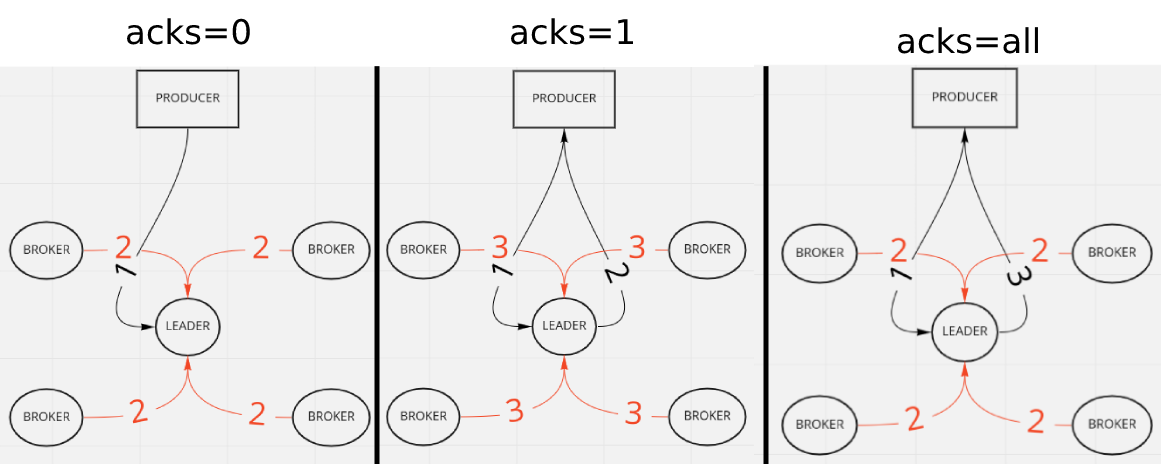
\includegraphics[width=17cm]{acks}
        \caption{}
        \label{fig:}
    \end{figure}

    Разумно будет считать, что параметр $acks$ будет определять, находятся ли данные в системе. Причём, полную уверенность в том, что данные пришли, мы можем получить лишь если отправка производилась с параметром $acks=all$ и сервер успешно ответил нам о том, что данные были записаны и отреплецированы.

    Будем считать настоящим data loss (true data loss) тот случай, когда отправитель получил ответ от сервера об
    успешной записи, но при этом, при последующем чтении, мы обнаружили, что эти данные отсутствуют.

    С acks=0 вроде бы все понятно. Здесь мы вообще не можем ничего гарантировать. Поэтому, такой случай действительно
    не интересен. Здесь нельзя говорить о потере данных. Такую систему сложно обвинить в неконсистентности, но легко в бестолковости.

    Теперь что касается acks=1. Здесь мы можем легко получить потерю данных. Алгоритм очень прост. Если мы записали на
    лидера сообщение, лидер ответил нам успехом, а реплики пока не торопятся синхронизироваться, может случиться так,
    что лидер упадет. Поскольку прошло не более $replica.lag.time.max.ms$ времени (этот конфигурационный параметр
    брокера отвечает за то, сколько времени должно пройти без синхронизаций, прежде чем лидер перестанет считать
    фолловера ISR) фолловеры остались ISR, можем выбрать нового лидера (несмотря на то, что на этих фолловерах лежат
    устаревшие данные, не хватает нашего сообщения)

    \section*{Тест 1. Внезапное падение лидера с acks=1}

    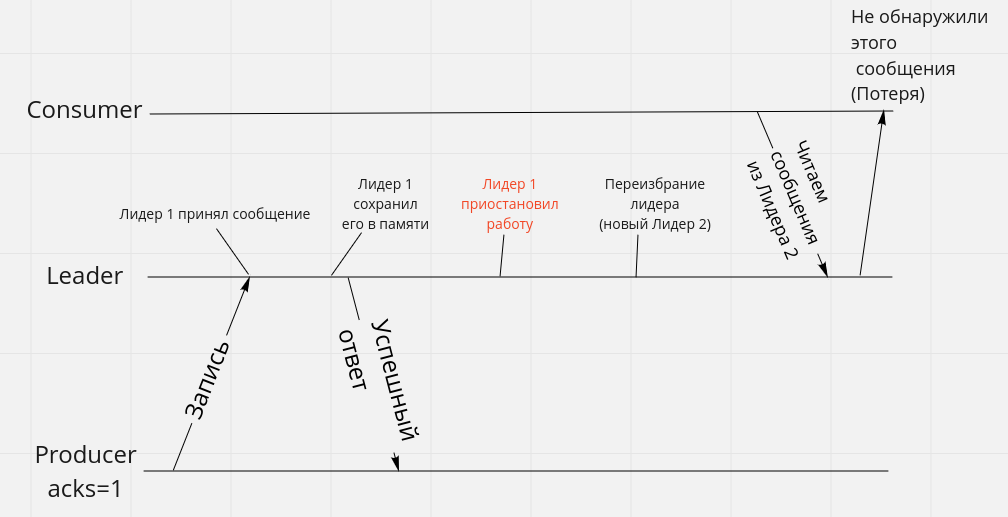
\includegraphics[width=15cm]{test1diag}

    ЦЕЛЬ: Показать, что внезапное падение лидера при acks=1 может привести к пропаже доставленного сообщения из системы.

    МЕТОД: В течении некоторого времени отправляем сообщения в Кафку, после чего внезапно останавливаем работу лидера.

    НАБЛЮДЕНИЯ: Был получен следующий результат: лидер ответил, что запись в Кафку прошла
    успешно. Но потом, в момент чтения, сообщение не было обнаружено.

    ОБЪЯСНЕНИЕ: Реплики приходят на лидера собирать данные с некоторой периодичностью. Когда лидеру пришло сообщение
    от продьюсера, он сделал запись к себе в файл, отправил продьюсеру успешный ответ. Но реплики еще не пришли к
    лидеру, чтобы обновить данные, это произойдет спустя некоторое время. Они остаются ISR все это время. И
    когда лидер внезапно останавливает работу, происходит переизбрание, мы выбираем нового лидера среди реплик, которые
    являются ISR. Реплика, избранная новым лидером, не имеет отправленного нами сообщения, поскольку на момент
    остановки предыдущего лидера репликация ещё не произошла. Прочитав из этой реплики, мы закономерным образом не
    обнаружим этого сообщения.

    \subsection{Вывод}
    Параметр acks=1 обладает недостатком. Мы не можем быть наверняка уверены, что сообщений было доставлено и
    осталось в системе, опираясь лишь на ответ системы.
    

    \section{Тест 2. Внезапное падение лидера с acks=all}
    Случай 1:

    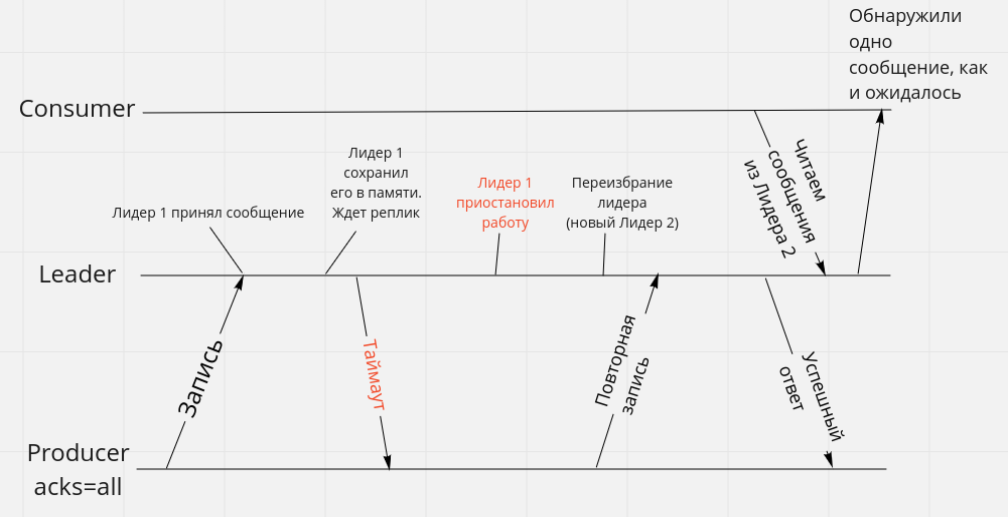
\includegraphics[width=15cm]{test2}

    Случай 2:

    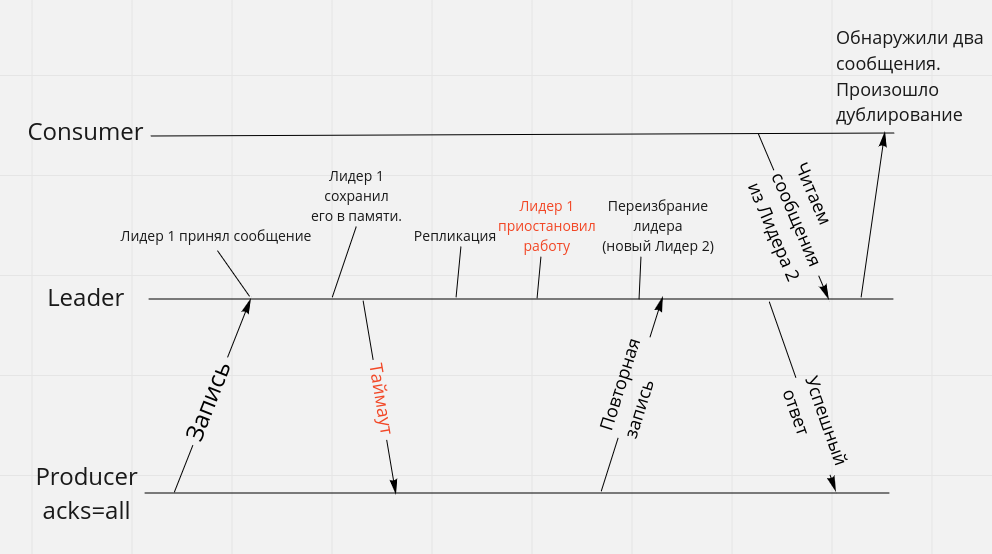
\includegraphics[width=15cm]{test22}

    ЦЕЛЬ: Показать, что acks=all решает проблему пропажи сообщения из системы при внезапной остановке работы лидера.

    МЕТОД: В течении некоторого времени отправляем сообщения в Кафку, после чего внезапно останавливаем работу лидера.

    НАБЛЮДЕНИЯ: Не было потерь сообщений. Однако встретилось дублирование сообщений.

    ОБЪЯСНЕНИЕ: Пропажа сообщений в первом тесте возникала именно по той причине, что лидер отвечал на запись успехом
    до того, как все брокеры отреплецируются. Это приводило к нарушению консистентности в распределенной системе.
    acks=all не даст лидеру слишком скоро ответить нам успехом.

    Дублирование же могло возникнуть из-за ретраев (повторная попытка отправить сообщение в случае неуспеха).
    Сценарий выглядит следующим образом:

    1) Лидер получил сообщение, записал к себе.

    2) Реплики отреплецировали его.

    3) Лидер остановил работу, не успев сообщить продьюсеру об успешной записи.

    4) Продьюсер ожидал слишком долго, случился таймаут.

    5) Продьюсер попробовал осуществить повторную запись, на что получил успех.

    6) В системе оказалось два одинаковых сообщения.


    \subsection{Вывод}
    acks=all позволяет нам избежать пропажи сообщений, но может приводить к их дублированию.

    \subsection{Случай с acks=all}
    Что касается acks=all, здесь намного сложнее придумать ситуацию, при которой что-то могло бы пойти не так.

    В крайнем случае, лидер просто не вернёт нам никакого ответа, что будет значить, что что-то пошло не так, сообщение не записано. Но всё ли так просто? На самом деле нет. И в этот раз нужно подумать вот о чём.

    Если в случае acks=1 нам пришёл ответ, мы едва ли можем быть уверенны в  том, что сообщение по-настоящему записалось в систему, что было подтвержено предыдущим тестом.

    Если же нам пришёл положительный ответ в случае acks=all, то будем считать, что ничего не предвещает опасности. (система гарантирует, что данные отреплецированы по всем репликам и не осталось реплики, в которой они были бы старыми, за исключением тех реплик, которые перестали быть in-sync в силу того, что не смогли быть отреплецированы, но эти реплики более не являются участниками топика, то есть не способны оказать вредное влияние на нашу систему. Мы не читаем из этих реплик, пока они не синхронизируются с лидером и не станут in-sync)

    Все реплики знают о наших данных, лидер знает о наших данных - всё чудесно. Но что значит отсутствие ответа при acks=all? Да и вообще, какой вывод мы можем сделать, если нам не пришёл ответ? Стоит подумать об этом.
    \newpage

    \section{Тест 3. Внезапное падение лидера с acks=all без ретраев}

    Случай 1:

    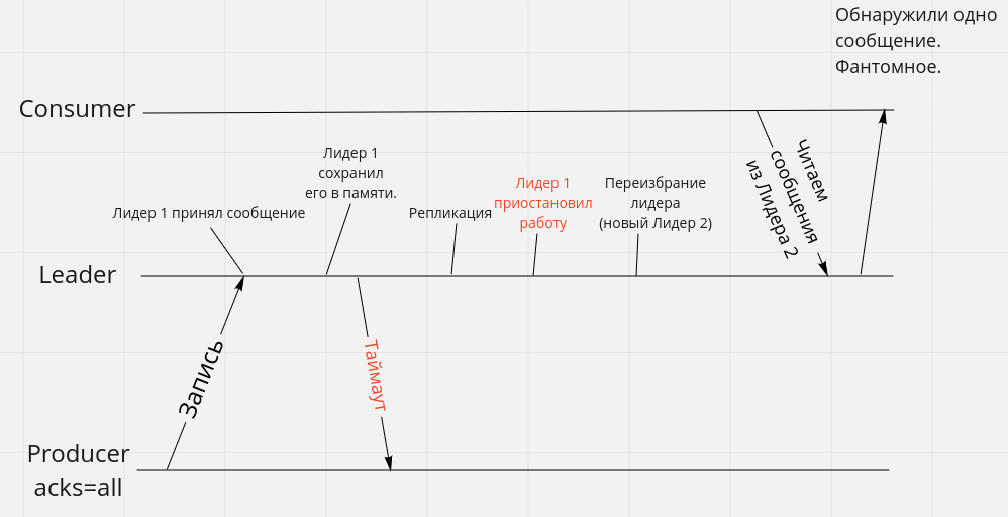
\includegraphics[width=15cm]{test3}

    Случай 2:

    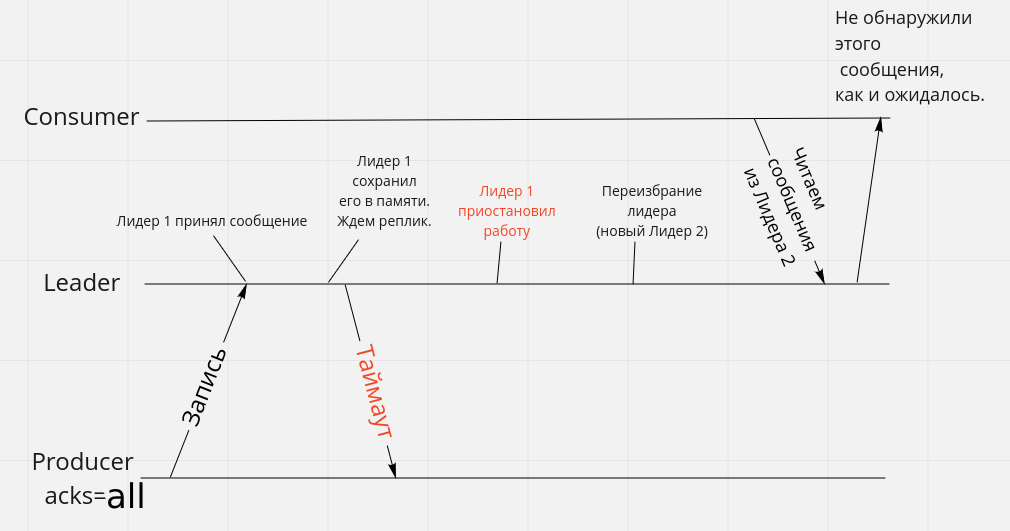
\includegraphics[width=15cm]{test333}


    ЦЕЛЬ: убедиться в том, что конфигурационный параметр продьюсера message.send.max.retries приводит к дублированию
    сообщений в топике.

    МЕТОД: изменим конфигурационный параметр на 0 и проделаем действия из второго теста.

    НАБЛЮДЕНИЯ: Дублирования данных не обнаружилось, фантомных записей тоже.

    ОБЪЯСНЕНИЕ: В момент падения лидера сообщение было в системе. Продьюсер, несмотря на безуспешный ответ, не
    попытался совершить повторную запись. С его точки зрения сообщение не было доставлено в систему. Однако в системе
    имеется сообщение, а значит мы имеем фантомную запись.

    \section{Важность конфигурирования таймаутов}
    Одна из проблем, которая может возникнуть при неправильно настроенных таймаутах - фантомные сообщения. Идея
    состоит в том, что продьюсер может не дождаться, прежде чем реплики синхронизируются.

    Интерес представляют следующие параметры:

    $replica.lag.time.max.ms$ - максимальное время, которое реплика может не синхронизироваться, оставаясь ISR.

    $replica.fetch.min.bytes$ - минимальный объем байт изменений, который должен произойти на лидере, чтобы реплика
    синхронизировалась.

    $replica.fetch.wait.max.ms$ - спустя это время, даже если байт изменений недостаточно, реплика все равно пойдет
    синхронизироваться.

    \section{Тест 4. Слишком долгое время синхронизации в сравнении с таймаутом продьюсера}

    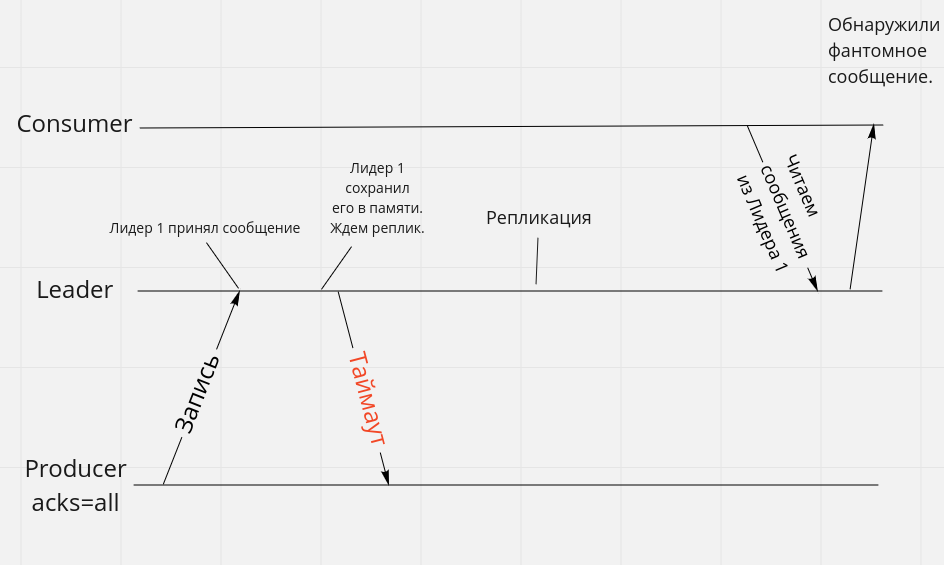
\includegraphics[width=15cm]{test4}

    ЦЕЛЬ: Показать, что слишком долгое время синхронизации в сравнении с таймаутом продьюсера может привести к
    возникнованию дублирующихся сообщений.

    МЕТОД: Мы должны получить ситуацию, когда время ожидания ответа от лидера на продьюсере закончится
    прежде чем все реплики успеют синхронизироваться, и лидер сообщит нам об удачной записи.
    
    Это достигается при следующих условиях:
    
        1) replica.fetch.wait.max.ms > producer timeout
            Если это будет не так, реплики синхронизируются до истечения времени ожидания, и мы получим успешный ответ.
    
        2) replica.lag.time.max.ms > replica.fetch.wait.max.ms
            Если это будет не так, метрика перестанет быть ISR, прежде чем данные отреплецируются, и лидер вернет нам
            успешный ответ.
    
        3) replica.fetch.min.bytes > размер сообщения
           Если это будет не так, реплика, получив слишком большое сообщение, сразу же пойдет реплецироваться.
           Поэтому, параметр replica.fetch.min.bytes необходимо сделать достаточно большим.
    
    НАБЛЮДЕНИЯ: Из 10 попыток записать ни одна не завершилась успехом. При этом при последующем чтении все 10
    сообщений обнаружились в системе.

    ОБЪЯСНЕНИЕ: Продьюсер записал на лидера, но тот не отвечал, поскольку реплики синхронизировались слишком долго.
    У продьюсера срабатывал таймаут, он начинал отправку следующего сообщения.

    \section{Exactly Once Delivery}
    Вообще говоря, порядок доставки сообщений - тоже данные, некоторое ординальное число, которое может быть искажено
    . Но в рамках данной работы хотелось бы заострять внимание на порядке доставки сообщений, а сосредоточиться на
    содержимом. Будем считать ради простоты, что топик - неупорядоченное множество. Намного интереснее было бы сосредоточить свое внимание на проблеме доставки.

    Проблема состоит в том, что наличие положительного ответа о записи от системы является критерием, а acks=all обеспечивает лишь достаточность наличия данных (то есть с параметром acks=all нам достаточно положительного ответа, чтобы быть уверенными, что данные оказались в системе, но наличие такого ответа, вообще говоря, не является необходимостью). То есть, отсутствие ответа о записи должно означать, что данных в системе нет.

    Лидеру приходят данные, нужно записать. Он записал, отреплецировал, отправил ответ, но, к сожалению, ответ потерялся. Мы думаем - наверное что-то пошло не так, отправляем данные ещё раз. Но на самом деле данные вполне таки записались, даже отреплецировались.

    Или другая ситуация: сервер записал данные, отреплецировал. Хотел было отправить пакет, но произошла какая-то непредвиденная ситуация, сервер упал - и продьюсер понятия не имеет о том, что пакет был успешно записан и отреплецирован.

    В общем, отсутствие ответа от сервера - не может гарантировать ничего. Мы не можем знать, записались ли данные или нет. Именно поэтому, как только мы не получили от сервера ответа, мы не можем принять решение о том, как действовать дальше: попробовать записать данные ещё раз, или ничего не делать. Можно, конечно, пойти и проверять самостоятельно, оказались данные на сервере или нет, но это оверхед.

    Эта проблема называется Exactly once delivery. В противовес exactly once стратегии имеются стратегии at-least-once и at-most-once.

    При at-least-once мы отправляем на брокера сообщения до тех пор, пока не получим удовлетворительный ответ. Таким образом там может накопиться сколь угодно много сообщений, но хотя бы одно будет, что для нас особенно важно. Это отражено в случае с acks=all и ретраями.

    При at-most-once мы просто один раз отправляем сообщение. Оно может не дойти, но мы уверены в том, что в нашем хранилище не окажется более двух таких одинаковых сообщений. Это имеет смысл, когда полное отсутствие каких-то данных в кафке намного лучше, чем несколько таких реквестов (например если речь идет о банковских операциях, намного лучше, если операция вообще не пройдет, чем если пройдет дважды). Здесь речь об acks=1 и ретраями.

    \subsection{Как решается проблема с Exactly Once Delivery}
    Очевидным образом, Exactly Once Delivery - невозможно.

    Доказательство здесь крайне простое. Базируется на той идее, что при записи в систему мы ожидаем получить от нее
    сообщение, ибо без такого сообщения не можем сделать вывод о том, что запись произошла, и остановиться. Но
    отсутствие такого сообщения не может значить ничего, как было сказано ранее.
    Если такое происходит, мы уже не можем придумать алгоритм, который бы позволил принять решение, как действовать дальше. Этот алгоритм во всяком случае требовал бы от нас спросить у системы, дошло ли до неё сообщение. Но будем считать, что субъектом доставки является доставщик, который лишь умеет генерировать новые сообщения и получать ответы. Как решить проблему?

    Решение на поверхности. Если отправка сообщения это некоторое отображение состояния системы, то почему бы не сделать это отображение идемпотентным, а затем исходить из кейса at-least-once delivery, то есть acks=all и ретраи.

    \subsection{Идемпотентность в кафке}
    На самом деле есть некоторое продолжение идеи Exactly Once Delivery. Называется Exactly Once Processing.

    Мы едва ли можем обеспечить точно одну доставку, но у нас есть возможность сказать системе то, что ей не следует обрабатывать дважды одно и то же сообщение. Именно это позволяет получить флаг $enable.idempotence = true$.

    \section{Тест 5. Внезапное падение лидера с acks=all с идемпотентностью}

    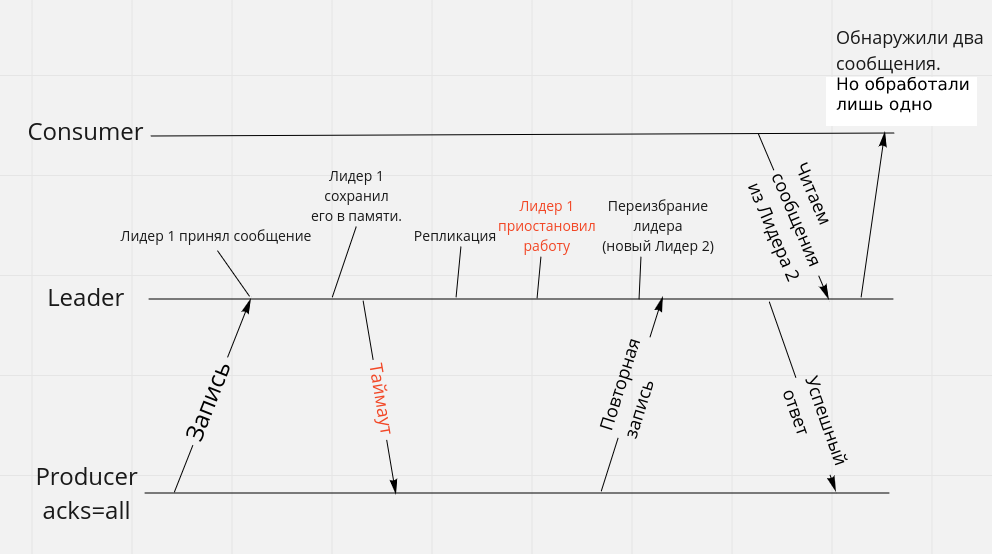
\includegraphics[width=15cm]{test5}

    ЦЕЛЬ: проверить, что идемпотентность позволяет избежать дублирования при ретраях и acks=all

    МЕТОД: включить идемпотентность, ретраи и поставить acks=all

    НАБЛЮДЕНИЯ: В тесте не удалось получить дублирования при включенном параметре enable.idempotence = true. Также не
    удалось обнаружить отсутствие. Можно сделать вывод, что флаг idempotence=true с acks=all и с множеством retry
    обеспечивает высокую устойчивость системы Kafka к аномалиям доставки сообщений при падении лидера партиции.

    \subsection{Недостатки идемпотентности.}

    В статье\cite{k7} приводятся причины, почему идемпотентность в Кафке - это не всегда хорошо. Дело в том, что
    из-за идемпотентности сообщения могут стать крайне тяжеловесными. Это может быть незаметно, относительно, если
    сообщения большие. Но если система заточена на обработку большого числа маленьких сообщений, то идемпотентность
    может существенно понизить пропускную способность системы.

    \section{Результаты:}
    В табличке:

        LAG = replica.lag.time.max.ms

        WAIT = replica.fetch.wait.max.ms

        BYTES = replica.fetch.min.bytes

        ФЗ = Фантомные сообщения

        ДД = Дублирование сообщений

        ПД = Потерянные данные

        С = Стоимость отправки сообщений

    \begin{center}
        \begin{tabular}{ c c c c c c c c c c c }
                  & acks & retries & WAIT & BYTES & LAG & И &
                  ФЗ & ДД & ПД & С  \\
                  TEST1 & 1 & true & > timeout & low & > timeout & false & false & true & true & low \\
                  TEST2 & all & true & > timeout & low & > timeout & false  & true & false & false & normal \\
                  TEST3 & all & false & > timeout & low & > timeout  & false & false & true & false & normal \\
                  TEST4 & all & false & < timeout & very high & < timeout & false  & false & true & false & normal \\
                  TEST4 & all & false & > timeout & low & > timeout & true  & false & false & false & high \\
        \end{tabular}
    \end{center}

    Таким образом, можно заключить, что проблема доставки сообщений не является такой уж тривиальной, имеет множество
    деталей, которые следует учитывать. В различных конфигурациях в системе Kafka возникают различные проблемы,
    связанные с доставкой сообщений. Конфигурация способна сильно повлиять на то, как будет
    проходить доставка сообщений. Например подходы at-least-once и at-most-once являются принципиально различными. В
    первой у нас есть
    гарантия
    того, что сообщение будет доставлено, во второй такой гарантии нет.

    И что немаловажно, не существует идеально конфигурации, такого набора параметров, который бы не имел недостатков.
    В процессе настройки распределенной системы всегда будут возникать выборы между двумя несовместимыми
    свойствами.
    \begin{thebibliography}{name}
        \bibitem{k1}
        Репозиторий

        Kafka клиент для JVM

        https://mvnrepository.com/artifact/org.apache.kafka
        \bibitem{k2}
        Статья

        Vivek Sinha, Kafka Exactly Once Semantics: 7 Critical Aspects

        https://hevodata.com/blog/kafka-exactly-once-semantics/
        \bibitem{k3} https://kafka.apache.org/documentation/

        Документация Apache Kafka

        \bibitem{k4}
        Репозиторий

        Исходный код Apache Kafka

        https://github.com/apache/kafka

        \bibitem{k5}
        Статья

        Neha Narkhede, Hands-Free Kafka Replication: A Lesson in Operational Simplicity

        https://www.confluent.io/blog/hands-free-kafka-replication-a-lesson-in-operational-simplicity/
        \bibitem{k6}
        Доклад

        Aphyr, Jepsen: Kafka

        https://aphyr.com/posts/293-jepsen-kafka

        \bibitem{k7}

        Статья

        Jack Vanlightly, Apache Kafka Idempotent Producer - Avoiding message duplication

        https://www.cloudkarafka.com/blog/apache-kafka-idempotent-producer-avoiding-message-duplication.html

        \bibitem{k8}

        Доклад

        Григорий Кошелев, Как готовить Кафку, чтобы не пригорало

        https://www.youtube.com/watch?v=M3HTM81P-Sg
        \bibitem{k9}

        Доклад

        Григорий Кошелев, Когда всё пошло по Кафке

        https://www.youtube.com/watch?v=A\_yUaPARv8U
        \bibitem{k10}
        Доклад

        Григорий Кошелев, Когда всё пошло по Кафке 2: Разгоняем продьюсеров

        https://www.youtube.com/watch?v=zMLfxztAVlo
    \end{thebibliography}
\end{document}